%%%%%%%%%%%%%%%%%%%%%%%%%%%%%%%%%%%%%%%%%%%%%%%%%%%%%%%%%%%%%%%%%%%%%%%%
% Plantilla TFG/TFM
% Escuela Politécnica Superior de la Universidad de Alicante
% Realizado por: Jose Manuel Requena Plens
% Contacto: info@jmrplens.com / Telegram:@jmrplens
%%%%%%%%%%%%%%%%%%%%%%%%%%%%%%%%%%%%%%%%%%%%%%%%%%%%%%%%%%%%%%%%%%%%%%%%

\chapter{Desarrollo}
\label{desarrollo}

La construcción de un sistema inteligente para la búsqueda y gestión de archivos personales requiere la integración de diversas tecnologías y herramientas consolidadas en el ámbito del desarrollo de software y la inteligencia artificial. Este capítulo tiene como objetivo, en una primera parte, revisar el estado del arte de los componentes tecnológicos clave que se han considerado para la implementación del presente proyecto. Posteriormente, en una segunda parte, se detallarán las decisiones de diseño finales para cada componente, justificando la elección, describiendo aspectos relevantes de su implementación y los desafíos encontrados durante el desarrollo.

\section{Estudio de Tecnologías}
\label{sec:estudio_tecnologias}
En esta sección se analizarán diferentes opciones en áreas fundamentales como la orquestación de tareas, la detección de cambios en el sistema de archivos, las soluciones de bases de datos para el almacenamiento de metadatos y embeddings, la contenerización para el despliegue y, finalmente, los frameworks para el desarrollo de la interfaz de usuario.

\subsection{Orquestadores de tareas}
La gestión eficiente de flujos de trabajo complejos, especialmente aquellos que involucran procesamiento de datos y tareas de machine learning, es crucial para el sistema propuesto. Un orquestador de tareas permite automatizar, programar y monitorizar estas secuencias de operaciones.
Para el estudio de orquestadores de tareas, se han tenido en cuenta las siguientes fuentes:
\cite{noauthor_best_2024}
\cite{suspicious_dress_350_airflow_2024}

\subsubsection{Prefect}
Prefect se presenta como una moderna plataforma de orquestación de flujos de trabajo, escrita principalmente en Python. Está diseñada específicamente para permitir a los desarrolladores diseñar, programar, ejecutar y monitorizar pipelines de datos y flujos de machine learning de manera fiable y escalable, con un enfoque en la simplicidad y la experiencia del desarrollador \cite{noauthor_pythonic_nodate}.

\paragraph{Ventajas}
\begin{itemize}
    \item \textbf{Facilidad de uso:} Prefect ofrece una sintaxis intuitiva y una configuración sencilla, lo que facilita la definición y gestión de flujos de trabajo complejos.
    \item \textbf{Flexibilidad:} Permite la orquestación de tareas en entornos locales, en la nube o híbridos, adaptándose a diversas necesidades.
    \item \textbf{Monitoreo y gestión:} Incluye herramientas integradas para el monitoreo, registro y manejo de errores en tiempo real.
\end{itemize}

\paragraph{Desventajas}
\begin{itemize}
    \item \textbf{Madurez:} Aunque ha ganado popularidad, Prefect es relativamente nuevo en comparación con otras herramientas más consolidadas.
    \item \textbf{Comunidad:} Su comunidad es más pequeña, lo que puede limitar la disponibilidad de recursos y soporte.
\end{itemize}

\subsubsection{Kafka}
Apache Kafka es un sistema de mensajería distribuido de código abierto, reconocido por su alto rendimiento y capacidad para manejar flujos de datos en tiempo real. Aunque su función principal es la de broker de mensajes, a menudo se utiliza en arquitecturas complejas para desacoplar sistemas y como parte de pipelines de datos más amplios, pudiendo actuar como un componente en la orquestación de eventos \cite{noauthor_apache_nodate}.

\paragraph{Ventajas}
\begin{itemize}
    \item \textbf{Alto rendimiento:} Kafka es conocido por su capacidad para manejar grandes volúmenes de datos con baja latencia.
    \item \textbf{Escalabilidad:} Diseñado para escalar horizontalmente, puede manejar cargas de trabajo crecientes de manera eficiente.
    \item \textbf{Ecosistema robusto:} Cuenta con una amplia gama de herramientas y conectores que facilitan su integración con otros sistemas.
\end{itemize}

\paragraph{Desventajas}
\begin{itemize}
    \item \textbf{Complejidad:} La configuración y gestión de Kafka pueden ser complejas, especialmente para usuarios sin experiencia previa.
    \item \textbf{Requisitos de recursos:} Para un rendimiento óptimo, Kafka suele requerir una infraestructura robusta, lo que puede ser excesivo para proyectos más pequeños.
\end{itemize}

\subsubsection{Airflow}
Apache Airflow es una plataforma de código abierto ampliamente adoptada para la creación, programación y monitorización programática de flujos de trabajo. Originalmente desarrollada por Airbnb, permite definir flujos de trabajo como Grafos Acíclicos Dirigidos (DAGs) de tareas, utilizando Python para su definición \cite{noauthor_home_nodate}.

\paragraph{Ventajas}
\begin{itemize}
    \item \textbf{Popularidad y comunidad:} Amplia adopción y una comunidad activa que proporciona numerosos recursos y soporte.
    \item \textbf{Flexibilidad:} Permite la programación y monitoreo de flujos de trabajo complejos.
\end{itemize}

\paragraph{Desventajas}
\begin{itemize}
    \item \textbf{Curva de aprendizaje:} Puede ser complejo de configurar y requiere conocimientos avanzados para su implementación efectiva.
\end{itemize}

\subsection{Detección de cambios en el sistema de archivos}
Un componente esencial del sistema es la capacidad de detectar automáticamente la creación, modificación o eliminación de archivos. Esta funcionalidad desencadena el proceso de análisis.

\subsubsection{Python}
Python, debido a su versatilidad y extenso ecosistema de bibliotecas, ofrece múltiples opciones.
\begin{itemize}
    \item \textbf{Watchdogs:} Biblioteca multiplataforma para observar eventos del sistema de archivos \cite{noauthor_watchdog_nodate}.
    \item \textbf{pyinotify:} Wrapper de Python para la API inotify de Linux (no portable).
    \item \textbf{inotify-simple:} Wrapper más sencillo para inotify de Linux.
    \item \textbf{inotifyx:} Similar a pyinotify, para inotify de Linux.
    \item \textbf{Polling Methods:} Verificación periódica, menos eficiente.
\end{itemize}

\subsubsection{Node.js}
\begin{itemize}
    \item \textbf{chokidar:} Biblioteca popular y eficiente para Node.js, multiplataforma.
\end{itemize}

\subsubsection{Java}
\begin{itemize}
    \item \textbf{WatchService:} API integrada en Java (\gls{nio}) para monitoreo.
\end{itemize}

\subsubsection{C++/C/C\#}
\begin{itemize}
    \item \textbf{FileSystemWatcher:} En .NET (C\#). Para C/C++, APIs específicas del SO (inotify en Linux, ReadDirectoryChangesW en Windows).
\end{itemize}

\subsubsection{Go}
\begin{itemize}
    \item \textbf{fsnotify:} Biblioteca popular en Go, interfaz común sobre APIs específicas.
\end{itemize}

\subsubsection{Rust}
\begin{itemize}
    \item \textbf{notify:} Biblioteca de Rust multiplataforma.
\end{itemize}

\subsection{Bases de datos}
El almacenamiento persistente de metadatos y embeddings es fundamental.

\subsubsection{Relacional}
Adecuadas para datos estructurados y consistencia \gls{acid}.

\paragraph{SQLite}
Autocontenida, sin servidor, transaccional. Almacena la base de datos en un único archivo \cite{noauthor_sqlite_nodate}.
\subparagraph{Ventajas}
\begin{itemize}
    \item \textbf{Ligereza y simplicidad.}
    \item \textbf{Portabilidad.}
    \item \textbf{Rendimiento en entornos de bajo recurso.}
\end{itemize}
\subparagraph{Desventajas}
\begin{itemize}
    \item \textbf{Concurrencia limitada en escrituras.}
    \item \textbf{Escalabilidad limitada.}
\end{itemize}

\paragraph{MariaDB}
Fork de MySQL, de código abierto.
\subparagraph{Ventajas}
\begin{itemize}
    \item \textbf{Rendimiento y escalabilidad.}
    \item \textbf{Compatibilidad con MySQL.}
    \item \textbf{Soporte para almacenamiento en columnas.}
\end{itemize}
\subparagraph{Desventajas}
\begin{itemize}
    \item \textbf{Complejidad en la configuración.}
    \item \textbf{Requisitos de recursos.}
\end{itemize}

\subsubsection{No relacional (NoSQL)}
Modelos de datos flexibles, escalabilidad horizontal.

\paragraph{MongoDB}
Orientada a documentos (\gls{bson}) \cite{noauthor_mongodb_nodate}.
\subparagraph{Ventajas}
\begin{itemize}
    \item \textbf{Flexibilidad del esquema.}
    \item \textbf{Escalabilidad horizontal.}
    \item \textbf{Alto rendimiento en lectura/escritura.}
\end{itemize}
\subparagraph{Desventajas}
\begin{itemize}
    \item \textbf{Consumo de recursos.}
    \item \textbf{Soporte limitado para transacciones complejas (tradicionales).}
\end{itemize}

\paragraph{ChromaDB}
Base de datos vectorial de código abierto para aplicaciones de \gls{ia}.
\subparagraph{Ventajas}
\begin{itemize}
    \item \textbf{Especializada en embeddings.}
    \item \textbf{Facilidad de uso y API intuitiva (Python).}
    \item \textbf{Integraciones con ecosistema de \gls{ia} (LangChain, LlamaIndex).}
    \item \textbf{Ligera y embebible.}
    \item \textbf{Código abierto.}
\end{itemize}
\subparagraph{Desventajas}
\begin{itemize}
    \item \textbf{Madurez y escalabilidad para producción masiva (en comparación).}
    \item \textbf{Funcionalidades de BD tradicional limitadas.}
    \item \textbf{Operaciones y gestión avanzada (para gran escala).}
\end{itemize}

\subsection{Contenerización}
La contenerización garantiza consistencia entre entornos. Docker es la plataforma líder.
\subsubsection{Docker}
Plataforma para automatizar el despliegue de aplicaciones en contenedores \cite{noauthor_home_0800}.
\paragraph{Ventajas}
\begin{itemize}
    \item \textbf{Portabilidad.}
    \item \textbf{Aislamiento.}
    \item \textbf{Facilidad de despliegue.}
\end{itemize}
\paragraph{Desventajas}
\begin{itemize}
    \item \textbf{Consumo de recursos (capa adicional).}
    \item \textbf{Complejidad adicional (gestión de contenedores).}
\end{itemize}

\subsection{Frameworks de Interfaz de Usuario}
La elección del framework impacta la experiencia del usuario y el desarrollo.

\subsubsection{Angular}
Framework de Google basado en TypeScript, completo y opinado.
\paragraph{Ventajas}
\begin{itemize}
    \item \textbf{Framework completo.}
    \item \textbf{Arquitectura estructurada.}
\end{itemize}
\paragraph{Desventajas}
\begin{itemize}
    \item \textbf{Curva de aprendizaje pronunciada.}
    \item \textbf{Complejidad innecesaria para proyectos simples.}
\end{itemize}

\subsubsection{React}
Biblioteca de JavaScript de Meta para construir UIs.
\paragraph{Ventajas}
\begin{itemize}
    \item \textbf{Biblioteca flexible.}
    \item \textbf{Amplia comunidad y recursos.}
\end{itemize}
\paragraph{Desventajas}
\begin{itemize}
    \item \textbf{Necesidad de configuraciones adicionales (para routing, estado global).}
\end{itemize}

\subsubsection{Vue.js}
Framework de JavaScript progresivo y accesible.
\paragraph{Ventajas}
\begin{itemize}
    \item \textbf{Simplicidad y facilidad de uso.}
    \item \textbf{Flexibilidad.}
\end{itemize}
\paragraph{Desventajas}
\begin{itemize}
    \item \textbf{Menor adopción en grandes empresas (en comparación).}
\end{itemize}

\subsubsection{Astro}
Framework web moderno para sitios rápidos y centrados en contenido (arquitectura de "islas").
\paragraph{Ventajas}
\begin{itemize}
    \item \textbf{Optimización para contenido estático y rendimiento.}
    \item \textbf{Integración con otros frameworks.}
\end{itemize}
\paragraph{Desventajas}
\begin{itemize}
    \item \textbf{Menor madurez para aplicaciones altamente interactivas.}
    \item \textbf{Ecosistema en crecimiento.}
\end{itemize}

\clearpage
\section{Decisiones de Diseño e Implementación}
\label{sec:decisiones_implementacion}
Tras el estudio de las tecnologías disponibles, en esta sección se detallan las herramientas finalmente seleccionadas para cada componente del sistema, justificando la elección, describiendo los aspectos más relevantes de su implementación y los problemas o consideraciones que surgieron durante el proceso de desarrollo.

\subsection{Orquestador de Tareas: Prefect}
\label{subsec:decision_prefect}
\subsubsection{Decisión y Justificación}
Para la orquestación de las tareas de procesamiento de archivos, extracción de metadatos, generación de embeddings y su posterior almacenamiento, se ha seleccionado \textbf{Prefect}. La elección se fundamenta en su enfoque moderno, su facilidad de uso al estar escrito en Python, lenguaje principal del proyecto, y su adecuada capacidad para gestionar pipelines de datos y de \gls{ml}. Aunque herramientas como Kafka ofrecen un rendimiento superior para flujos de datos masivos y Airflow cuenta con una comunidad más extensa, Prefect proporciona un equilibrio óptimo entre simplicidad, flexibilidad y potencia para las necesidades específicas de este proyecto. Su curva de aprendizaje es más accesible en comparación con Airflow, y su infraestructura requerida es menos exigente que la de Kafka, haciéndolo idóneo para un proyecto de esta envergadura.

\subsubsection{Implementación}
La implementación con Prefect se estructura en torno a \textit{Tasks} (tareas individuales) y \textit{Flows} (flujos de trabajo que orquestan las tareas).

Las principales \textbf{Tasks} definidas son:
\begin{itemize}
    \item \texttt{summarize\_text}: Resume el texto proporcionado como parámetro.
    \item \texttt{analyze\_image}: Analiza el contenido de una imagen utilizando un modelo multimodal (en este caso, Gemma).
    \item \texttt{get\_image\_metadata}: Extrae metadatos específicos de archivos de imagen.
    \item \texttt{rag\_query}: Procesa una consulta del usuario (\textit{query}) utilizando un modelo de lenguaje grande (\gls{llm}), en este caso Mistral, enriqueciendo la consulta con resultados de búsqueda vectorial obtenidos de ChromaDB para generar una respuesta contextualizada.
    \item \texttt{rag\_query\_with\_db}: Realiza una búsqueda de similitud en ChromaDB basada en la consulta del usuario, devolviendo un número máximo especificado de coincidencias.
\end{itemize}

Estos \textit{tasks} se orquestan en los siguientes \textbf{Flows}:
\begin{itemize}
    \item \texttt{new\_file}: Se activa al detectar un nuevo archivo en la carpeta monitorizada. Este flujo gestiona la detección de duplicados, la identificación del tipo de archivo, la extracción de metadatos, la generación de embeddings y el almacenamiento de los resultados en ChromaDB.
    \item \texttt{modified\_file}: Opera de manera similar a \texttt{new\_file}, pero se desencadena cuando un archivo existente es modificado. En este caso, se actualizan los metadatos y los embeddings en ChromaDB si el hash del contenido del archivo ha cambiado, indicando una modificación sustancial.
    \item \texttt{deleted\_file}: Se activa tras la eliminación de un archivo. Procede a eliminar el documento correspondiente y sus metadatos asociados de ChromaDB.
    \item \texttt{process\_query}: Se inicia cuando el usuario realiza una búsqueda a través de la interfaz. Genera los embeddings de la consulta, los envía a ChromaDB para encontrar coincidencias semánticas, y los resultados se proporcionan a un \gls{llm} para generar una respuesta elaborada.
\end{itemize}

Si bien Prefect ofrece capacidades robustas para la ejecución paralela de tareas y flujos, en la implementación actual, el grado de paralelización se ve limitado por los recursos computacionales disponibles en un entorno de desarrollo local. Tareas intensivas como la generación de embeddings o las inferencias de modelos \gls{llm} pueden ser costosas. En un entorno de producción con un servidor adecuadamente dimensionado (con mayor capacidad de \gls{cpu}, \gls{gpu} y \gls{ram}), se podría explotar de manera mucho más efectiva la paralelización para procesar múltiples archivos o consultas simultáneamente, mejorando significativamente el rendimiento y la capacidad de respuesta del sistema.

La Figura \ref{fig:prefect_dashboard} muestra una vista general del dashboard de Prefect, donde se pueden monitorizar los flujos y tareas.

\begin{figure}[!htbp]
    \centering
    
\includegraphics[width=0.9\textwidth]{archivos/prefect.png}
    \caption{Dashboard principal de Prefect para la monitorización de flujos.}
    \label{fig:prefect_dashboard}
\end{figure}

\subsection{Detección de Cambios: Python con Watchdogs}
\label{subsec:decision_watchdogs}
\subsubsection{Decisión y Justificación}
La detección de cambios en el sistema de archivos se ha implementado utilizando \textbf{Python} en combinación con la biblioteca \textbf{watchdogs}. Esta elección se basa en la naturaleza multiplataforma de \texttt{watchdogs}, crucial para una aplicación destinada a la gestión de archivos personales que podría ejecutarse en diversos sistemas operativos. Python, como lenguaje principal del proyecto, facilita la integración de este componente con el resto del sistema, especialmente con el orquestador de tareas Prefect.

\subsubsection{Implementación}
Se ha desarrollado un script de Python que utiliza \texttt{watchdogs} para monitorizar de forma recursiva un directorio específico proporcionado por el usuario, centrándose exclusivamente en archivos. El script implementa un manejador de eventos personalizado, subclase de \texttt{FileSystemEventHandler}, que reacciona a los eventos de creación (\texttt{on\_created}), modificación (\texttt{on\_modified}) y eliminación (\texttt{on\_deleted}) de archivos. Al detectar un evento relevante, el script desencadena el flujo de Prefect correspondiente. Adicionalmente, al iniciar el programa, se realiza un análisis exhaustivo inicial de toda la carpeta asignada; durante este proceso, los archivos duplicados o aquellos ya procesados y sin cambios significativos se gestionarán eficientemente gracias al sistema de detección de duplicados basado en hashes, evitando reprocesamientos innecesarios.

Un desafío particular surgió con la detección de archivos modificados en tiempo real, especialmente en sistemas Windows. Este sistema operativo tiende a realizar pequeñas modificaciones en los metadatos de los archivos al abrirlos o copiarlos, lo que provocaba activaciones múltiples y no deseadas del evento \texttt{on\_modified} para un mismo archivo en cortos periodos. Para mitigar este comportamiento, se implementó una caché en memoria que almacena temporalmente información sobre los archivos recientemente procesados por eventos en tiempo real. Esta caché ayuda a prevenir la reactivación innecesaria de flujos para eventos de modificación que no representan cambios sustanciales en el contenido, optimizando el rendimiento.

Es importante destacar que este script de detección de cambios se ejecuta en un hilo separado para no bloquear la operatividad del resto del sistema. Además, se ha diseñado para ignorar eventos relacionados con directorios en su creación o modificación, procesando únicamente archivos. En el caso de la eliminación (\texttt{on\_deleted}), dado que el objeto del sistema de archivos ya no existe en el momento de la notificación, no se realiza una comprobación para distinguir entre archivo y directorio, asumiendo que el flujo de Prefect manejará adecuadamente la solicitud de eliminación en la base de datos si el ID (basado en la ruta) existiera.

\subsubsection{Detección de Duplicados}
La detección de duplicados se basa en el cálculo de un hash SHA256 del contenido del archivo que se almacena como metadato en ChromaDB. Cuando se detecta un nuevo archivo, se calcula su hash y se consulta en la base de datos para verificar si ya existe un embedding con ese hash, lo que indicaría que el archivo ya ha sido procesado previamente y por ende, que está duplicado. Si el hash ya existe, se omite el procesamiento del archivo y se evita la creación de un nuevo embedding, optimizando así el uso de recursos y el almacenamiento.

\subsection{Base de Datos: ChromaDB}
\label{subsec:decision_chromadb}
\subsubsection{Decisión y Justificación}
Para el almacenamiento de metadatos y, de forma crucial, los embeddings vectoriales generados por los modelos de \gls{ia}, se ha optado por \textbf{ChromaDB}. Inicialmente, se consideró SQLite por su simplicidad para el almacenamiento de metadatos básicos, y de hecho, se desarrolló un controlador para esta base de datos que permanece disponible en el código base como alternativa o complemento futuro. Sin embargo, la funcionalidad central del sistema reside en la capacidad de realizar búsquedas semánticas eficientes basadas en embeddings, lo que hizo de una base de datos vectorial la elección más adecuada.

ChromaDB fue seleccionada por su especialización en el manejo de embeddings, su facilidad de uso a través de su API Python y su capacidad para operar de forma ligera y embebible, características ideales para el desarrollo y despliegue de este proyecto.

\subsubsection{Implementación}
ChromaDB se utiliza para almacenar dos tipos principales de información por cada archivo procesado, organizados en una "colección":
\begin{itemize}
    \item \textbf{Embeddings:} Vectores numéricos densos que representan el contenido semántico del archivo, permitiendo búsquedas por similitud.
    \item \textbf{Metadatos:} ChromaDB permite asociar un diccionario de metadatos a cada embedding. En este proyecto, se almacenan, como mínimo, los siguientes campos, aunque cada tipo de archivo puede añadir metadatos específicos adicionales:
        \begin{itemize}
            \item \texttt{path}: La ruta absoluta original del archivo en el sistema de archivos.
            \item \texttt{filename}: El nombre del archivo con su extensión.
            \item \texttt{size}: El tamaño del archivo en bytes.
            \item \texttt{creation\_time}: La fecha y hora de creación del archivo.
            \item \texttt{hash}: Un hash SHA256 del contenido del archivo. Este metadato es crucial para evitar el procesamiento y almacenamiento duplicado de archivos idénticos, incluso si tienen nombres o ubicaciones diferentes. Antes de procesar un nuevo archivo, se calcula su hash y se consulta en ChromaDB si ya existe un embedding con ese mismo \texttt{hash} en sus metadatos.
        \end{itemize}
\end{itemize}
Las búsquedas semánticas se realizan enviando un vector de embedding (generado a partir de la consulta del usuario) a ChromaDB, que devuelve los `k` embeddings más similares junto con sus metadatos asociados. Actualmente, el valor de `k` se ha limitado a 3 resultados por consulta. Esta restricción se debe principalmente a las limitaciones de la ventana de contexto de los modelos de \gls{llm} que se ejecutan localmente, ya que un mayor número de resultados (y por ende, más texto para procesar) podría exceder dicha ventana o degradar significativamente el rendimiento. Esta limitación podría mitigarse en el futuro con el uso de modelos de \gls{llm} más avanzados que soporten ventanas de contexto mayores o mediante el acceso a recursos computacionales más potentes.

El controlador de ChromaDB implementado se encarga de gestionar la conexión, la creación de colecciones si no existen, y las operaciones CRUD (inserción, lectura, actualización y eliminación) de embeddings y metadatos. Incluye funciones para verificar si un archivo ya ha sido procesado (basándose en su hash) y para actualizar los datos si se detectan modificaciones.

Una decisión de diseño importante fue utilizar el campo de metadatos de ChromaDB para almacenar toda la información descriptiva del archivo, incluyendo el hash. Esto evita la necesidad de una base de datos relacional adicional (como SQLite) para la gestión de metadatos y la detección de duplicados, simplificando la arquitectura y aprovechando la eficiencia de ChromaDB para consultas basadas en estos metadatos.

\subsubsection{Consideraciones Futuras}
La arquitectura modular del sistema, con componentes bien definidos (backend API, motor de Prefect, detector de cambios), está diseñada para facilitar una futura migración a contenedores. Si el proyecto evolucionara hacia un despliegue en entornos más complejos, multiusuario o en la nube, la adopción de Docker (posiblemente junto con Docker Compose) sería un paso lógico y altamente recomendable. Esto permitiría empaquetar el servidor de la API, el agente de Prefect, la base de datos (especialmente si se optara por una versión servida de ChromaDB o una alternativa) y la interfaz de usuario en contenedores separados y orquestados, mejorando la escalabilidad y la mantenibilidad.

\subsection{Interfaz de Usuario: Vue.js}
\label{subsec:decision_vue}
\subsubsection{Decisión y Justificación}
Para el desarrollo de la interfaz de usuario (\gls{ui}), se ha seleccionado \textbf{Vue.js}. La principal razón detrás de esta elección fue la búsqueda de simplicidad y una curva de aprendizaje accesible, dado que la \gls{ui}, aunque importante para la interacción del usuario, no constituye el núcleo de innovación del proyecto, el cual está centrado en la inteligencia artificial y la gestión de archivos del backend.

Aunque existía una mayor familiaridad previa con Angular por parte del desarrollador, su complejidad inherente y su estructura altamente opinada se consideraron excesivas para las necesidades de la interfaz de este proyecto. Vue.js ofrece un excelente equilibrio entre funcionalidad y facilidad de desarrollo, permitiendo construir una interfaz reactiva y moderna sin la sobrecarga asociada a frameworks más robustos y extensos.

\subsubsection{Implementación}
La interfaz de usuario desarrollada con Vue.js se comunica con un backend implementado en Flask (Python), el cual actúa como intermediario para interactuar con Prefect y ChromaDB. Las funcionalidades principales implementadas en la \gls{ui} incluyen:
\begin{itemize}
    \item Un campo de búsqueda central donde el usuario puede introducir sus consultas en lenguaje natural.
    \item Visualización clara y ordenada de los resultados de la búsqueda, mostrando la ruta y si procede una miniatura del archivo.
    \item Una sección de configuración que permite al usuario modificar el Host y el puerto del Backend, cambiar el modelo de \gls{ia} utilizado para la respuesta final y la temperatura de la respuesta generada por el \gls{llm} y un botón para reinciar el chat.
    \item Una vista de "explorador de archivos" que permite navegar por los archivos ya procesados por el sistema.
\end{itemize}
La aplicación se ha estructurado sobre un único componente por comodidad ya que es una web sencilla y se ha puesto especial atención en crear una interfaz amigable y acogedora. Por ejemplo, se utilizan "emoticonos" en mensajes iniciales o de ayuda, una estrategia observada en plataformas orientadas al cliente, como el soporte de Amazon, con el fin de hacer la experiencia del usuario más agradable al interactuar con lo que se pretende sea un "asistente inteligente" para los archivos del usuario final.

El principal desafío durante la implementación fue la curva de aprendizaje inicial de Vue.js, al no ser el framework con el que se tenía mayor experiencia previa. Se priorizó una funcionalidad básica pero robusta, dejando posibles mejoras estéticas avanzadas o funcionalidades secundarias de la \gls{ui} para futuras iteraciones, dado el enfoque del proyecto en la funcionalidad del backend.

Las Figuras \ref{fig:front_home}, \ref{fig:front_config} y \ref{fig:front_explorer} muestran diferentes pantallas de la interfaz de usuario desarrollada.

\begin{figure}[!htbp]
    \centering
    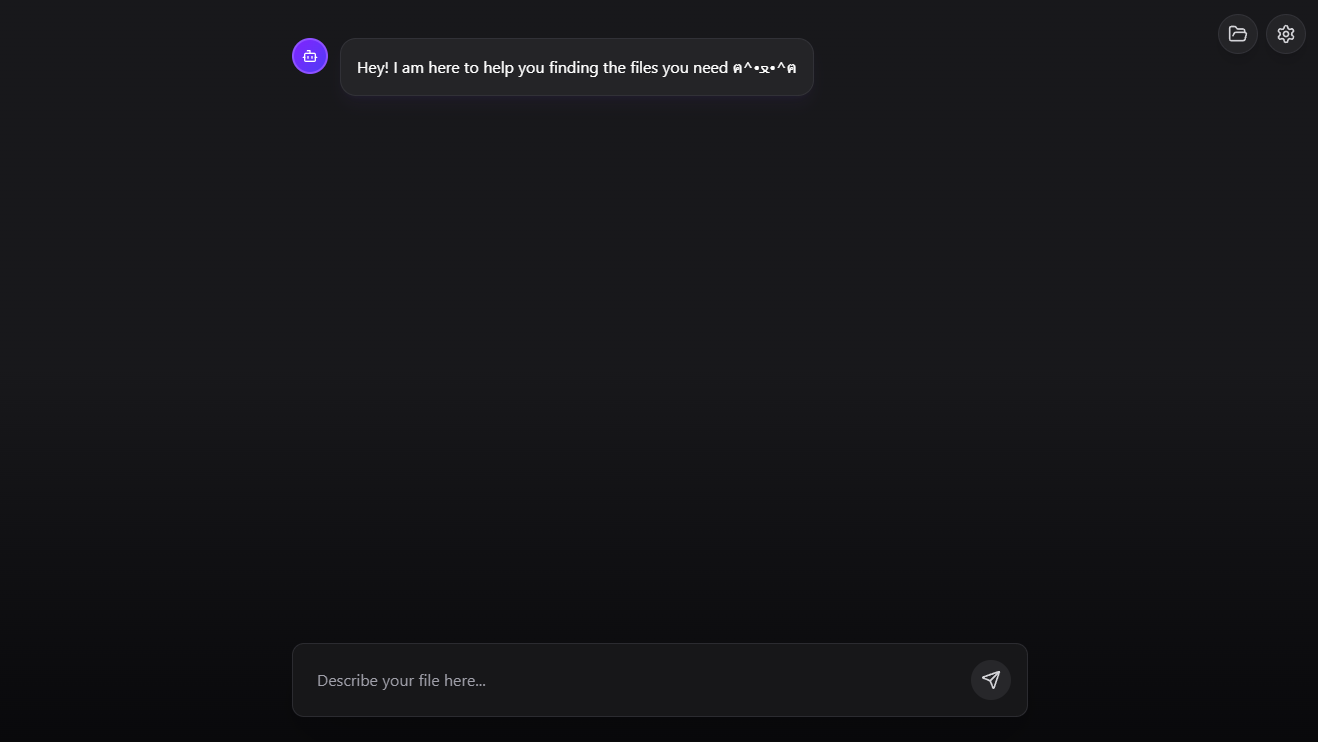
\includegraphics[width=0.8\textwidth]{archivos/front_home.png}
    \caption{Pantalla principal de la interfaz de usuario, con el campo de búsqueda.}
    \label{fig:front_home}
\end{figure}

\begin{figure}[!htbp]
    \centering
    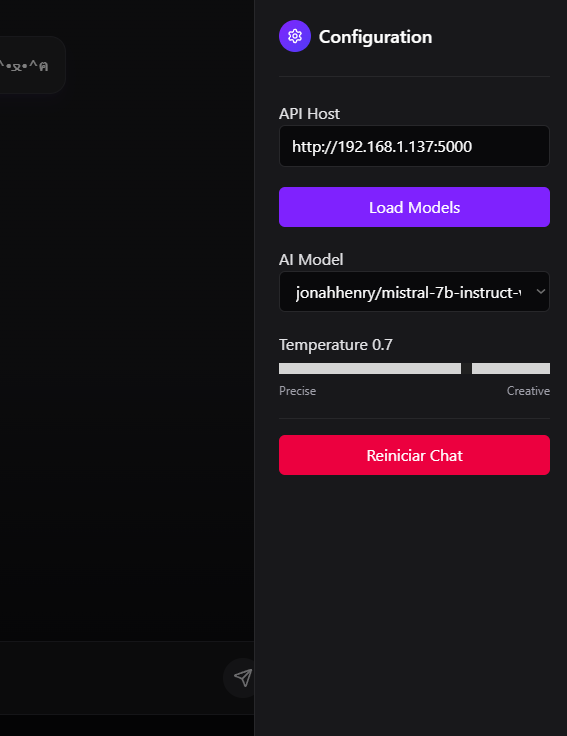
\includegraphics[width=0.6\textwidth]{archivos/front_config.png}
    \caption{Apartado de configuración de la interfaz de usuario.}
    \label{fig:front_config}
\end{figure}

\begin{figure}[!htbp]
    \centering
    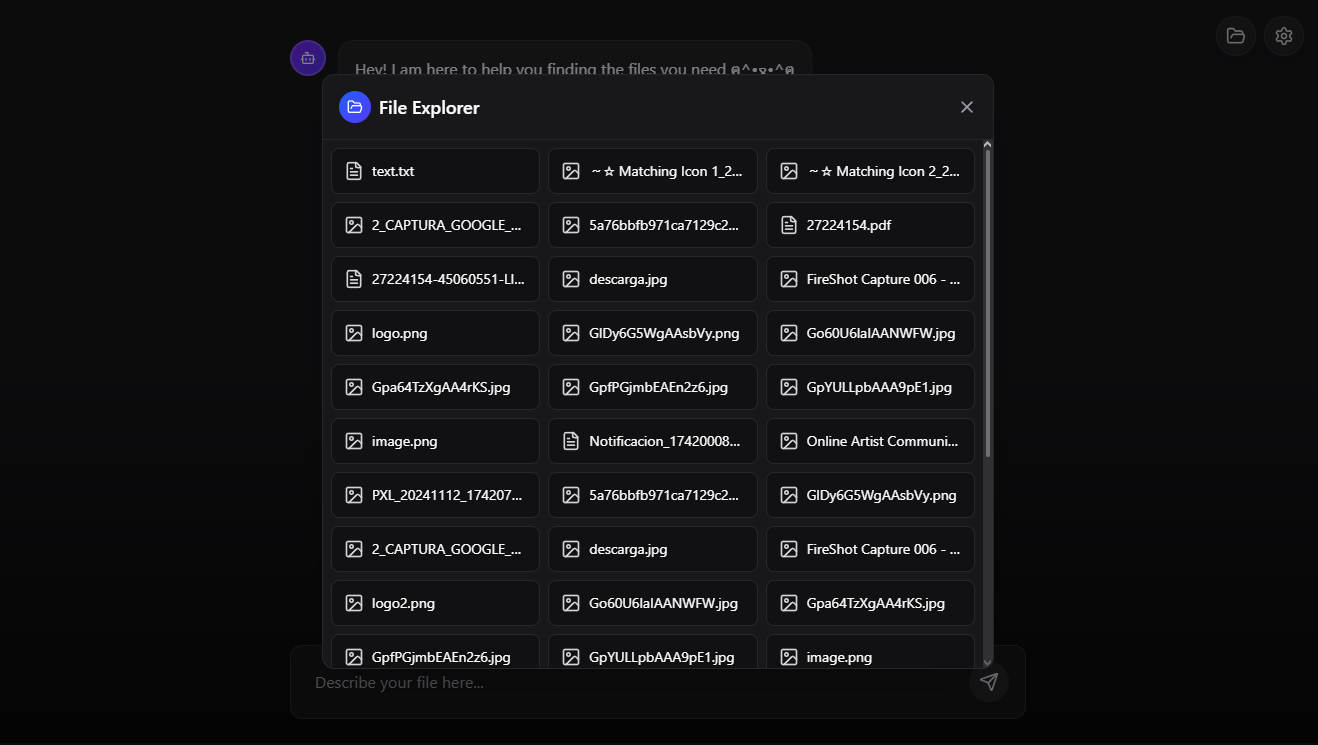
\includegraphics[width=0.7\textwidth]{archivos/front_explorer.png}
    \caption{Pantalla del explorador de archivos procesados.}
    \label{fig:front_explorer}
\end{figure}

\subsection{API REST: Flask}
\label{subsec:decision_api}
\subsubsection{Decisión y Justificación}
Para la comunicación entre el frontend (Vue.js) y los servicios del backend (Prefect, ChromaDB, lógica de negocio), se ha optado por desarrollar una API RESTful utilizando \textbf{Flask} en Python. Esta elección se basa en la simplicidad, ligereza y flexibilidad de Flask, que permite crear rápidamente endpoints bien definidos. Al ser Python el lenguaje principal del proyecto, Flask facilita una integración natural con los demás componentes del backend.

\subsubsection{Implementación}
El servidor Flask se ha configurado para servir tanto la API REST como los archivos estáticos de la aplicación Vue.js (generados tras el proceso de compilación de Vue). Los principales endpoints de la API incluyen:
\begin{itemize}
    \item \texttt{/api/status}: Proporciona información sobre el estado general del sistema, como la cantidad de archivos procesados o el estado de los servicios de monitorización.
    \item \texttt{/api/models}: Devuelve información sobre los modelos de \gls{ia} configurados y disponibles para el procesamiento de consultas o análisis de archivos.
    \item \texttt{/api/query}: Recibe las consultas de búsqueda textuales del usuario desde la interfaz, las procesa y las reenvía al flujo de Prefect correspondiente para obtener resultados de ChromaDB y la respuesta generada por el \gls{llm}.
    \item \texttt{/api/path\_descs}: Permite obtener una lista de todos los archivos que han sido procesados y están indexados en el sistema, con metadatos básicos.
    \item \texttt{/api/file\_content}: Dado la ruta de un archivo de imagen, devuelve su contenido para ser visualizado en la interfaz.
    \item \texttt{/api/file\_details}: Proporciona la descripción y los metadatos detallados de un archivo identificado por su ruta.
\end{itemize}
Se implementó \gls{cors} (Cross-Origin Resource Sharing) para permitir las solicitudes desde el servidor de desarrollo de Vue.js al servidor Flask durante la fase de desarrollo. Un desafío grande fue la gestión del estado y la sincronización de la información para el endpoint \texttt{/api/status}, asegurando que refleje de manera precisa y actualizada el estado de los diversos componentes del sistema.

\subsection{Gestión de Modelos de IA: LMStudio}
\label{subsec:decision_lmstudio}
\subsubsection{Decisión y Justificación}
Para la gestión y ejecución local de los modelos de lenguaje grande (\gls{llm}) y modelos multimodales, se ha optado por utilizar \textbf{LMStudio}~\cite{noauthor_lm_nodate}. La principal ventaja de LMStudio radica en su facilidad de uso: es una aplicación de escritorio que permite descargar, configurar y ejecutar una amplia variedad de modelos de \gls{ia} de código abierto (provenientes de plataformas como Hugging Face) a través de una interfaz gráfica intuitiva. Además, expone los modelos cargados a través de un servidor local compatible con la API de OpenAI, lo que simplifica enormemente la integración con el código Python del proyecto \cite{noauthor_lmstudio-python_nodate}.

La alternativa habría sido gestionar la descarga, configuración y ejecución de cada modelo directamente mediante bibliotecas de Python como `transformers` o `llama-cpp-python`. Si bien esto ofrecería un control más granular, también implicaría una mayor complejidad en el código y en el proceso de configuración inicial para el usuario final del proyecto por lo que se deja como una tarea a futuro cuando se plantee consolidar el producto.

\subsubsection{Implementación}
LMStudio se utiliza como un componente externo al código principal del proyecto. El usuario debe instalar LMStudio, descargar los modelos deseados y ejecutarlos a través del servidor local que provee la aplicación. El backend de Python del sistema se comunica con este servidor local de LMStudio mediante peticiones HTTP a los endpoints estándar de la API de OpenAI (e.g., \texttt{/v1/chat/completions} para \gls{llm} o \texttt{/v1/completions} para modelos que lo soporten, adaptándose según el modelo específico y su configuración en LMStudio).

Esta dependencia de un software externo implica que el usuario debe realizar estos pasos de configuración manualmente. No obstante, para el alcance de este proyecto, la simplificación en el desarrollo y la flexibilidad para probar diferentes modelos que ofrece LMStudio superan la desventaja de la configuración manual. En la documentación del proyecto se detallan los pasos para configurar LMStudio y los modelos recomendados.

\subsection{Contenerización: No implementada (Docker)}
\label{subsec:decision_docker}
\subsubsection{Decisión y Justificación}
Durante la fase de análisis, se evaluó la posibilidad de utilizar tecnologías de contenerización como \textbf{Docker}. Se reconocen plenamente sus ventajas en términos de reproducibilidad del entorno, aislamiento de dependencias y simplificación del despliegue en diferentes máquinas.

Sin embargo, para la etapa actual del proyecto, y como se anticipó en el análisis inicial, se ha optado por no implementar una solución de contenerización. Esta decisión se fundamenta en varios factores prácticos:
\begin{enumerate}
    \item El orquestador Prefect, en su modo de ejecución local, se instala fácilmente como un paquete Python y no requiere una configuración de servidor compleja para este proyecto.
    \item LMStudio, la herramienta seleccionada para la gestión y ejecución de los modelos de \gls{ia} locales, es una aplicación de escritorio con un instalador directo, diseñada para ser utilizada en el sistema operativo anfitrión.
    \item La gestión de dependencias de Python se ha manejado eficazmente mediante el uso de entornos virtuales (`venv`), asegurando un aislamiento adecuado a nivel de proyecto.
\end{enumerate}
Dado que el objetivo principal era validar la funcionalidad central del sistema en un entorno de desarrollo local, y los componentes clave no presentaban complejidades de entorno que justificaran la sobrecarga administrativa de Docker en esta fase, se consideró más ágil proceder sin él.

\subsection{Modelos de IA: Mistral y Gemma}
\label{subsec:decision_models}
Tras el estudio del arte, se ha optado por el modelo \textbf{\texttt{gemma-3-12b-it}} como la elección principal para las capacidades multimodales de LLMSearch en ejecución local. Las razones que sustentan esta decisión son:

\begin{enumerate}
    \item \textbf{Equilibrio entre Tamaño y Rendimiento Local:} Con 12 mil millones de parámetros, \texttt{gemma-3-12b-it} es lo suficientemente robusto para tareas de comprensión multimodal y RAG, sin imponer una carga computacional excesiva en sistemas de escritorio modernos, especialmente al considerar versiones cuantizadas (e.g., GGUF Q4\_K\_M) que son gestionadas eficientemente por LMStudio.
    \item \textbf{Capacidad Multimodal Inherente:} Al ser un modelo diseñado con la multimodalidad como característica central, se simplifica la arquitectura al no requerir la orquestación compleja de múltiples modelos especializados para visión y lenguaje por separado para la funcionalidad base.
    \item \textbf{Optimización para Instrucciones (`-it`):} La variante "instruct-tuned" está optimizada para seguir instrucciones y participar en diálogos de pregunta-respuesta, lo cual es fundamental para la interacción del usuario con el buscador.
    \item \textbf{Ecosistema Abierto y Soporte Local:} La naturaleza abierta de Gemma y su buen soporte en herramientas de ejecución local como LMStudio aseguran una mayor facilidad de implementación y experimentación para el usuario final del TFG.
\end{enumerate}

Si bien modelos más grandes como \texttt{gemma-3-27b-it} podrían ofrecer un rendimiento superior, sus requisitos de hardware son considerablemente mayores, lo que limitaría la aplicabilidad del sistema en un espectro más amplio de equipos personales. Por otro lado, aunque \texttt{mistral-7b-it} es excelente para texto, la integración nativa de multimodalidad en Gemma reduce la complejidad de desarrollo para la funcionalidad principal de LLMSearch. Por lo tanto, \texttt{gemma-3-12b-it} se presenta como la opción más pragmática y equilibrada para satisfacer los requisitos del proyecto en el contexto de un Trabajo Fin de Grado enfocado en la viabilidad y funcionalidad local.
Por otro lado se ha seleccionado \texttt{mistral-7b-it} como el modelo de \gls{llm} para la generación de respuestas a las consultas del usuario. Este modelo es conocido por su capacidad de generar texto coherente y relevante en una variedad de contextos, lo que lo convierte en una opción adecuada para el sistema de búsqueda semántica. Al igual que con Gemma, se ha optado por una versión cuantizada (GGUF Q4\_K\_M) para optimizar el rendimiento en hardware local.

Para el correcto funcionamiento de ambos modelos se han creado prompts específicos que guían al modelo en la generación de respuestas adecuadas. Estos prompts se han diseñado para maximizar la calidad de las respuestas generadas, teniendo en cuenta el contexto y la información proporcionada por el usuario y para evitar que el modelo se niegue a responder o genere respuestas irrelevantes.
Estos prompts se detallan en los Anexos Anexo \ref{anx:prompt_img_desc} y Anexo \ref{anx:prompt_verify}

\subsection{Interfaz de Línea de Comandos (CLI)}
\label{subsec:decision_terminal}
\subsubsection{Decisión y Justificación}
Además de la interfaz gráfica de usuario, se consideró útil proporcionar una interfaz de línea de comandos (CLI) para permitir interacciones básicas con el sistema, como realizar búsquedas o iniciar el proceso de monitorización. Esto puede ser ventajoso para usuarios avanzados, para la automatización de tareas mediante scripts o para entornos donde una GUI no está disponible o no es deseada. Se utilizó el ecosistema estándar de Python para empaquetar y distribuir esta CLI.

\begin{figure}[!htbp]
    \centering
    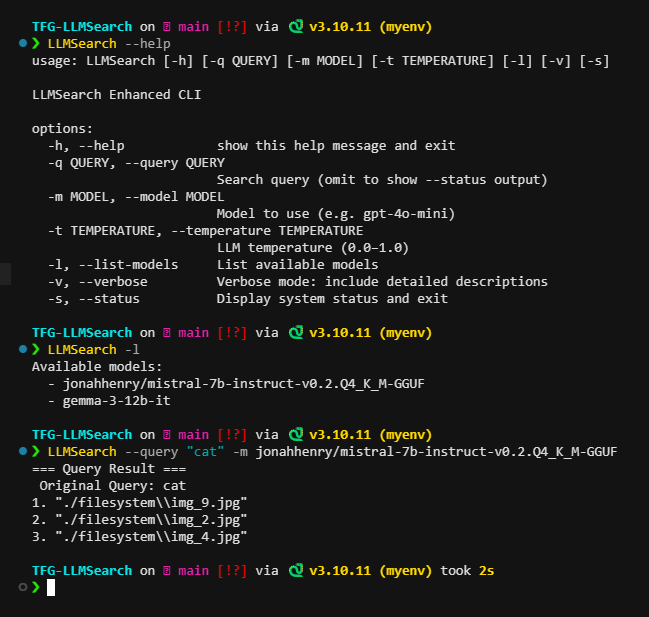
\includegraphics[width=0.7\textwidth]{archivos/terminal_example.png}
    \caption{Interfaz de línea de comandos (CLI) del sistema.}
    \label{fig:terminal}
\end{figure}

\subsubsection{Implementación}
Para crear un punto de entrada ejecutable desde la terminal, se ha utilizado la funcionalidad de \texttt{entry\_points} de \textbf{setuptools}, la biblioteca estándar de Python para la construcción y distribución de paquetes. Se definió un archivo \texttt{setup.py} (o \texttt{pyproject.toml} con la configuración equivalente) que incluye la siguiente configuración para los scripts de consola:

\begin{lstlisting}[language=Python, caption={Definición del punto de entrada en setup.py}, label=lst:setup_py_cli, basicstyle=\footnotesize\ttfamily, breaklines=true]
from setuptools import setup

setup(
    name="llmsearch",
    version="0.1",
    py_modules=["llmsearch"],
    entry_points={
        "console_scripts": [
            "LLMSearch=llmsearch:main",
        ],
    },
)
\end{lstlisting}
En el ejemplo anterior, existe un módulo Python llamado \texttt{llmsearch\_cli.py} que contiene una función \texttt{main()}. Esta función se encarga de parsear los argumentos proporcionados en la línea de comandos (utilizando bibliotecas como \texttt{argparse}) y de invocar la lógica correspondiente en el backend del sistema enviando una solicitud a la API REST.

Una vez instalado el paquete el usuario puede invocar la CLI desde cualquier ubicación en su terminal:
\begin{verbatim}
LLMSearch --help
LLMSearch --query "mapa del mundo"
\end{verbatim}
Esta aproximación ofrece una forma estándar y robusta de crear herramientas de línea de comandos en Python, facilitando la interacción del usuario con las funcionalidades principales del sistema sin depender exclusivamente de la interfaz web.